\renewcommand\evenpagerightmark{{\scshape\small Scale-up}}
\chapter[Scale-up]%
{Scale-up}
\label{Scale-up}

\section{Analysis of a non reactive flow in a basic case}

\begin{figure}[!h]
  \centering
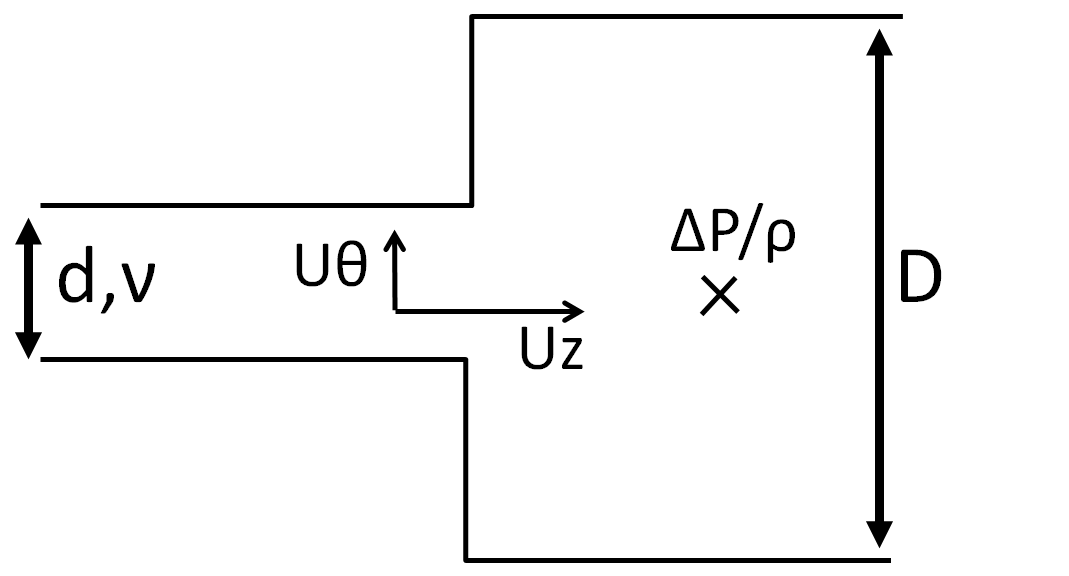
\includegraphics[width=0.6\textwidth]{fig/Schema_Vashy1.png}
  \caption{Basic case}
 \label{Vaschy1}
\end{figure}
Given a burner of internal diameter $d$, with a bulk velocity $u_{z}$,a tangential velocity $u_{\theta}$ ,  followed by a combustion chamber of internal diameter $D$, and a fluid with a kinematic viscosity $\nu$, we want to describe the behavior of the non-reactive flow inside the furnace. For instance, we can study the quantity $\frac{\Delta P}{\rho}$ at a given point inside the combustion chamber, we can otherwise choose $u_{r}$or any physical values, the adimensional numbers will be the same.

We need hypothesis for the velocities : let's assume a top-hat axial velocity, and a solid block body rotation, giving the shape :$u_{\theta}=\Omega r$. Let us use the Vaschy-Buckingham Theorem : we assume that the flow (through the quantity $\frac{\Delta P}{\rho}$ for example, or any else ) only depends on the previous data. 

Since we have 5 independent inputs ($d$,$\nu$,$u_{z}$,$\Omega$,$D$) with 2 units ($m$,$s$), there are $5-2=3$ adimensional numbers which fully describes the non-reactive flow. We can guess them, or find it back with linear analysis :
\begin{itemize}
\item $Re$ 
\item $S=\frac{\Omega d}{u_{z}}$
\item $C=\frac{d}{D}$
\end{itemize}

The adimensional number $\frac{\Omega d}{u_{z}}$ is written $S$ because we find, to within a constant, the well-known swirl-number :$S=\frac{\int_{0}^{d/2} u_{\theta} u_{z} r^2 dr}{d/2\int_{0}^{d/2}  u_{z}^2 r dr}$ 

Consequently, the flow is only a function of $S$, $Re$ and $C$ .

\paragraph{Influence of the density}

It has been a shortcut not to consider the density in the previous case. If we assume that the flows depends also on the density, let us enumerate the input parameters, we have now 6 of them : $d$,$\mu$,$\rho$,$u_{z}$,$\Omega$,$D$, but we also have added $kg$ as a unit. Hence, we have the same number of adimensional units : $6-3=3$. This is an important case where this powerful theorem demonstrates that there are simple cases where the kinematic viscosity is enough to describe the fluid.

\section{In the case of non uniform fields depending on cylindrical coordinates}

G\begin{figure}[!h]
  \centering
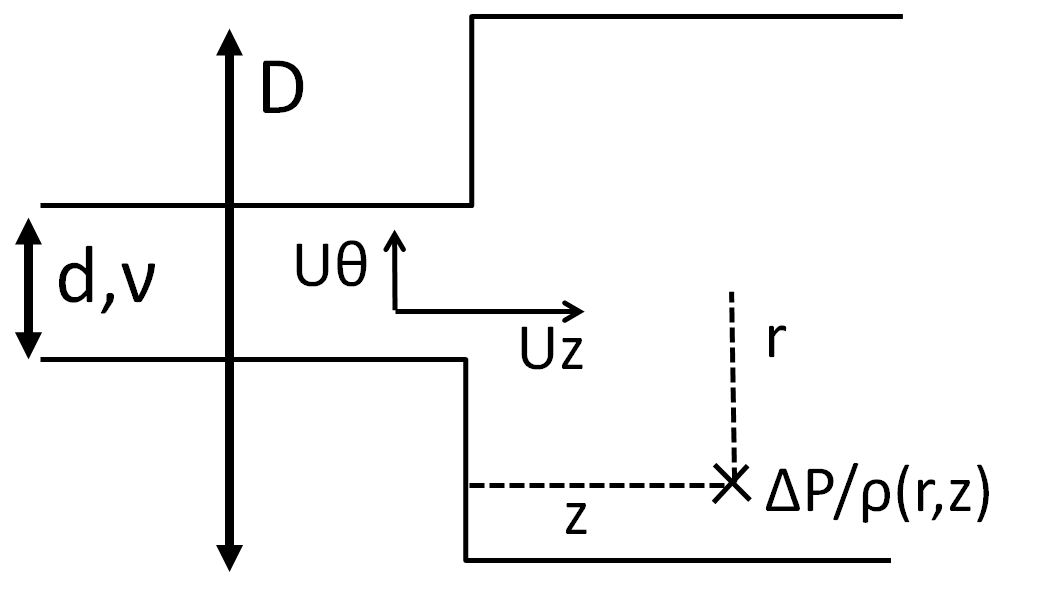
\includegraphics[width=0.6\textwidth]{fig/Schema_Vashy2.png}
  \caption{With cylindrical coordinates}
 \label{Vaschy2}
\end{figure}
In the previous case, the parameter $\frac{\Delta P}{\rho}$ has been considered as a macroscopic one, since not depending on $z$ and $r$ (let us assume the symmetry of rotation by neglecting $\theta$) . Let us now consider the case where we want to study a field depending on cylindrical coordinates : now $\frac{\Delta P}{\rho}(r,z)$. 

If we use the same approach, we easily see that there are 2 more unknown, with the same amounts of units, we have just added two adimensional coordinates to the problem, for instance $r/D$ and $z/D$. The input physical parameters driving the phenomena are the same. Hence, this is not absurd not to consider some coordinates, but we still have to know that the field will depend on adimensional coordinates.

Here, we have : $\frac{\Delta P}{\rho}(r,z)=f(\frac{r}{D},\frac{z}{D},Re,S,\frac{d}{D})$

From now on, let us not consider the dependency of the cylindrical coordinates.

\section{With a quarl angle}

Since Paul Jourdaine \cite{paul_jourdaine_nom_effect_2016} has now shown the huge dependency on the flow of the quarl angle, we can add it in our dimensional analysis.

\begin{figure}[!h]
  \centering
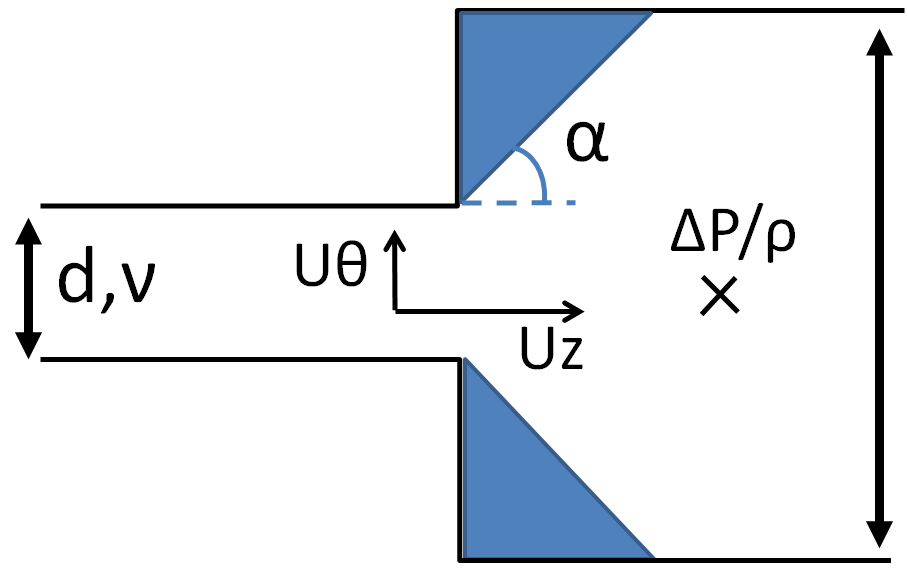
\includegraphics[width=0.6\textwidth]{fig/Schema_Vashy3.png}
  \caption{With quarl angle}
 \label{Vaschy3}
\end{figure}

The Vacshy-Buckingham analysis gives easily : that the quarl number is itself an adimen
sional number, we now have :
$\frac{\Delta P}{\rho}=f(\alpha,Re,S,\frac{d}{D})$

\section{Two coaxial swirled flows}

The new case deals with two flows, as presented in \ref{Vaschy4}. One common adimensional number we can find in the literature is the impulsion ratio : $J=\frac{\rho_{1} u_{1}^2}{\rho_{2} u_{2}^2}$ . In that case, one understands that the two densities will now influence the behavior of the flow. Thus, $\rho_{1}$ and $\rho_{2}$ must be counted on the inputs. We introduce here a new units, $kg$. 
\begin{figure}[!h]
  \centering
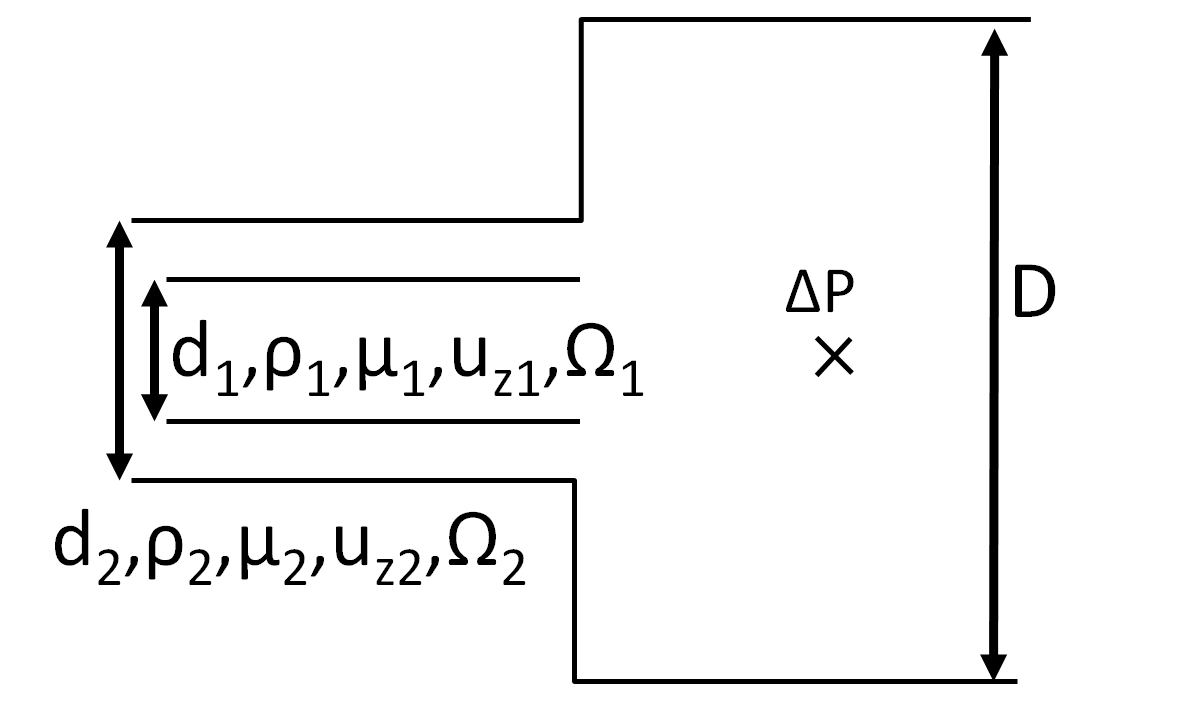
\includegraphics[width=0.6\textwidth]{fig/Schema_Vashy4.png}
  \caption{Two coaxial swirled flows}
 \label{Vaschy4}
\end{figure}
According to \ref{Vaschy4}, each flow at the inlet is fully described with the diameter $d$ (or equivalent diameter for the outer flow), the density $\rho$, the dynamic viscosity $\mu$ and the velocity flow (the axial velocity supposed as top-hat velocity $u_{z}$, and the tangential velocity supposed as solid block rotation, so that the vorticity $\Omega$ fully describes the tangential flow :  $u_{\theta}=\Omega r$). Hence, we have 5 input parameters for each flow, and the diameter $D$ of the combustion chamber. With 3 units ($m$,$kg$ and $s$), the Vaschy-Buckingham theorem gives that $11-3=8$ adimensional numbers fully describes the behavior of the flow :

Here are the chosen parameters : 

$Re_{1}$,$Re_{2}$,$S_{1}$,$S_{2}$,$\frac{d_{1}}{D}$,$\frac{d_{2}}{D}$,$J=\frac{\rho_{1} u_{z1}^2}{\rho_{z2} u_{2}^2}$,$\frac{\mu_{1}}{\mu_{2}}$. 

One can easily check that any new adimensional number is a combination of the previous ones : 

For instance, we could have chosen $\frac{u_{z1}}{u_{z2}}$ instead of $J$, but we have the relation : $J=\frac{Re_{1}}{Re_{2}} \cdot \frac{u_{z1}}{u_{z2}} \cdot \frac{\mu_{1}}{\mu_{2}}$ 

Hence, the non-reactive flow might be fully studied with a parametric study of these 8 adimensional numbers.

\section{Sizing of the strioscopy experiment}
\subsection{The approach}
As far as it is possible, we want the adimensional numbers to remain the same: $\frac{d_{1}}{D}$,$\frac{d_{2}}{D}$,$Re_{1}$,$Re_{2}$,$S_{1}$,$S_{2}$,$J$ and $\frac{\rho_{1}}{\rho_{2}}$. We also want to use the same velocities as the ones in HPPOX. 

According to our hypothesis to consider the geometrical swirl number, we see that the use of the same ATR-30norm burner automatically gives that $\frac{d_{1}}{D}$,$\frac{d_{2}}{D}$,$S_{1}$ and $S_{2}$ remain the same. (Let us neglect in a first approach the fact that we will not use any combustion chamber in the strioscopy diagnostic, so that the diameter $D$ is not defined anymore). 

Hence, we have to choose our inlet gases in order to keep as constant as possible the quantities : $Re_{1}$,$Re_{2}$,$J$ and $\frac{\rho_{1}}{\rho_{2}}$. Unfortunately, other conditions make the conservation of these adimensional quantities all the more difficult :
\begin{itemize}
\item To increase the efficiency of the strioscopy, one needs a high density gradient, implying that we need   $\frac{\rho_{2}}{\rho_{1}}$ far from the unity. "far" still needing to be defined. By heating air at $100^\circ C$, Y. Joumani (ref) had a density ratio of 1.27, which apparently was not enough. Fortunately, since we want to approach $\frac{\rho_{1}}{\rho_{2}}$ from the experiment on Calhory, the value reaches $\frac{\rho_{O_{2}}}{\rho_{CH_{4}}}_{Freiberg}=3$ , which may be enough to have useful density gradients.
\item Dealing with the experiment, heating the gases or diluting them make the experiment more difficult to implement. Particularly, though it would be an efficient solution, using natural gas without combustion chamber nor furnace seems unsafe.
\end{itemize}

\section{Sizing of the Calhory experiment}

\subsection{Overview}

The main difference is that the kinetic aspect also need to be considered here, since there the combustion phenomenon is now effective. The Vaschy-Buckingham analysis with a non-reactive flow  gave adimensional numbers to be conserved. It seems difficult to use the same approach to make kinetic adimensional numbers appear :

\begin{itemize}
\item There are many more unknown to the problems and free parameters (every fraction of each specie in each flow, and we are just adding the temperature as dimension
\item In order to use the Vaschy-Buckingham theorem, the main idea is to assume the parameters from the beginning that will be involved in a certain metric we want to observe. Here, non only the determination of the  involved parameters are exactly the scientific problem the internship wants to tackle, but also it is very hard to define a single metric to observe the flame (should it be the flame length, the width, the maximum temperature...?)
\end{itemize}
Consequently, the bibliography has been widely investigated in order to define the main parameters. Let us not forget that the idea is not the predict the flame length, but to make sure that the identified parameters are conserved between Freiberg and the Calhory experiment.

The simplest investigation is the laminar case : in (\# ref Veynante), the length of a diffusion flame in the laminar case is $L_{f}=\frac{e_{0}Re}{2\pi}\cdot \frac{1}{Z_{st}^2}$  with $e_{0}$ a geometrical length. We know in that a ratio of 40 will change the pressure, so the Reynolds $Re$, but Veynantes also says that the flame length in turbulence flow does not depend on the Reynolds. Hence, the important parameter here is $Z_{st}$, and it is the one we want to keep constant. According to (\#ref Peters), a clear definition of $Z_{st}$ can be : $Z_{st}=(1+\frac{\nu Y_{F,1}}{Y_{O_{2},2}})^{-1}$ where $\nu$ is the mass stoechiometric ratio (4 for $CH_{4}-O_{2}$ flame),    $Y_{F,1}$ the mass ratio of fuel in the fuel injection ($Y_{F,1}=1$ if it is pure $CH_{4}$) and $Y_{O_{2},2}$ the mass ratio of oxygen in the oxydant injection ($Y_{O_{2},2}=0.23$ if it is pure air).

Consequently, we choose the $Z_{st}$ to be constant. In Freiberg, $Z_{st}=0.31$.

\subsection{Reflexions for the scale-up}

The purpose of this section is to explain the strategy of the scale-up. One of the two main objectives of the internship is to establish general scale-up to investigate if the Freiberg industrial flame can be obtained without pressurized furnace and with complete combustion. The overall scale-up is based on the hypothesis of the internship : "The fluid mechanic mixture would drive the flame topology on 1st order, and the kinetic and heat transfer are of 2nd order."


The dimensional analysis and the literature review has permitted to investigate the quantities to be conserved. To resume, the following quantities has to remain constant between Freiberg and Calhory :
\begin{enumerate}
\item The geometry of the burner and the furnace
\item The impulsion ration $ J$
\item The  stoichiometric mixture fraction $Z_{st}$
\item the outer speed $u_{3}$
\item the inner speed $u_{1}$

\end{enumerate}
Then, the free parameters are :
\begin{enumerate}
\item the inner gas temperature, $T_{1}$
\item the outer gas temperature, $T_{3}$
\item the mass fraction of $CH_{4}$ in the inner injection : $Y_{CH_{4},1}$ (the rest being $N_{2}$)
\item  the mass fraction of $O_{2}$ in the outer injection : $Y_{O_{2},3}$(the rest being $N_{2}$ as well)
\item The pressure $P$
\end{enumerate}

Some new constraints reduces the number of degrees of liberty, since there are technological parameters of the Calhory furnace :
\begin{itemize}
\item The pressure $P$ is atmospheric
\item The air-ratio equivalence $\phi=\frac{\nu_{eq} \cdot \dot{m}_{CH_{4},1}}{\dot{m}_{O_{2},3}}$ is limited to $0.95$ : the combustion has to be complete (unfortunately, this is a very severe restriction, that will have to be overcome)
\item For practical reasons, it is way simpler if the outer composition of the gaz is only hot oxygen :  $Y_{O_{2},3}=1$ (fortunately, it is not an obstacle)
\item It is also way simpler that the temperature in the inner injection is ambiant temperature : $T_{1}=293K$.
\end{itemize}
"Way simpler" mostly implies that if that a simple technological option is not chosen, the deadlines of the intership will not be respected. 

Given those constraints, there can be a set of solution, an unique solution, or no solution, and compromises would have to be made.
 
 The following section shows that no solution can respect all the scale-up and practical contraints of the system. By accepting a slight modification of the inner speed $u_{1}$, a best solution can though be defined.
\subsection{Analysis of the scale-up}

There are several calculations to achieve, and efforts have be drawn to find the most direct way to determine the nominal point N.

\paragraph{Conservation of the stoichiometric fraction $Z_{st}$ }


The definition of Peters (\#ref peters) of stoichiometric mixture fraction results from jet theory. It is also well used in non-reactive flow to determine the precise line where the two elements of a mixture are at the stoichiometry. Consequently, the definition of $Zst$ can be generalized from Peters with :
\begin{equation}
Z_{st}=(\frac{\nu Y_{\chi,1}}{Y_{\tilde{\chi},3}}+1)^{-1}
\end{equation}
Where $Y_{\chi,1}$ is the mass fraction of the specie of interest $\chi$ in the inner injection (1), and $Y_{\tilde{\chi},3}$ the same for the specie $\tilde{\chi}$ in the outer injection (3). For the case of an inner injection of fuel ($\chi=CH_{4}$), and outer injection of oxydant ($\tilde{\chi}=O_{2}$), we fin the same definition as the one of peters. But this new definition of $Z_{st}$ if of particular relevance when examining the case of Freiberg flame : dealing with the mixture, there is an inversion of $\chi$ and $\tilde{\chi}$, so that we have :
\begin{equation}
Z_{st, Freiberg}=(\frac{\nu Y_{O_{2},1}}{Y_{CH_{4},3}}+1)^{-1}
\end{equation}
With $\nu=1/4$, corresponding to the respective stoichiometry. 
Consequently, if we want to conserve the stoichiometric fraction $Z_{st}$ on Calhory furnace, we have to choose on Calhory:
$\chi$ and $\tilde{\chi}$, so that we have :
\begin{equation}
(\frac{\nu Y_{CH_{4},1}}{Y_{O_{2},3}}+1)^{-1}=Z_{st, Freiberg}=0.6945
\end{equation}

Assuming that $Y_{O_{2},3}$ is fixed for practical reason ($=1$ in Calhory furnace). Consequently, $Y_{CH_{4},1}$ is fixed as well with :
\begin{equation}\label{eq:Zst_conservation}
Y_{CH_{4},1}=\frac{Y_{O_{2},3}}{\nu} (\frac{1}{Z_{st}}-1)
\end{equation}
Hence, the composition of the gaz in the inner injection is fully known. $T_{1}$ being set to $20^\circ C$, the volumic mass is set :
\begin{equation}
\rho_{1}=\frac{1}{1+Y_{CH_{4},1} (\frac{M_{N_{2}}}{M_{CH_{4}}}-1)} 
\frac{P M_{N_{2}}}{R T_{1}} 
\end{equation}
Inner speed $u_{1}$ is still considered as a free parameter, so the mass flow $\dot{m}_{1}$ in the inner injection is fully descibred.

In the outer injection, only the temperature $T_{3}$ is not fixed, we have as well :
\begin{equation}
\rho_{3}=\frac{1}{1-Y_{CO_{2},3} (1-\frac{M_{N_{2}}}{M_{O_{2}}})} 
\frac{P M_{N_{2}}}{R T_{3}} 
\end{equation}

\paragraph{The conservation of the impulsion ratio}
\newpage

\section{Investigation on Optisos analysis }

\subsection{Context of the investigation}

Given the lack of experimental data one is faced with in terms of ATR combustion. The experiments on Freiberg HP-POX burner are almost our only contact with industrial real results of combustion process in ATR burner. Furthermore, a detailed campaign has been made with parametric study of different inputs, such as the S/C ratio, the load variation or the Oxygen/NG velocity ratio. The chosen metric to investigate the flame topology here will be the flame length 

The conclusion of the report are that :
\begin{enumerate}
\item Changing the pressure of the ATR burner from 30 to 50 bars leads to small variation of the flame length
\item The S/C ratio is the parameter that the biggest impact on the flame topology : With a S/C ratio increasing from 1 to 1.4, the flame length decreases from 124mm to 84mm
\item The burner load also drives the flame length : increasing burner load shortens the flame
\item High temperatures of the reactor leads to longer flame
\end{enumerate}

In order to emphasize the conclusion of the reports, here are the corresponding plot from Optisos report :

\begin{figure}[h!]
  \centering
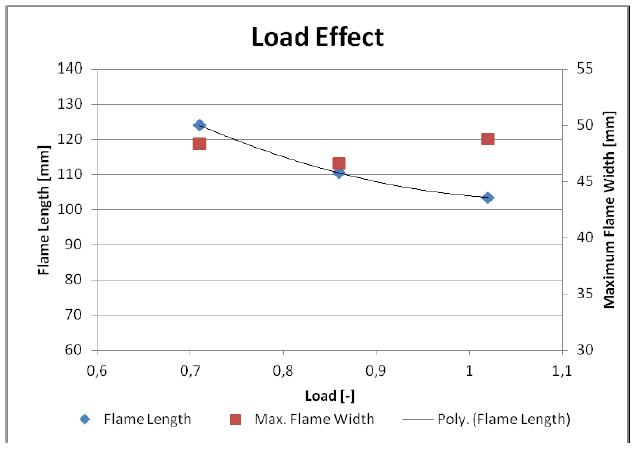
\includegraphics[width=0.45\textwidth]{fig/Optisos_Load_effect.PNG}
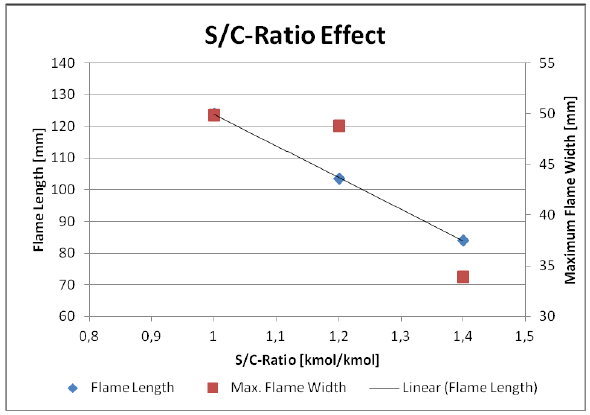
\includegraphics[width=0.45\textwidth]{fig/Optisos_S_C_effect.PNG}
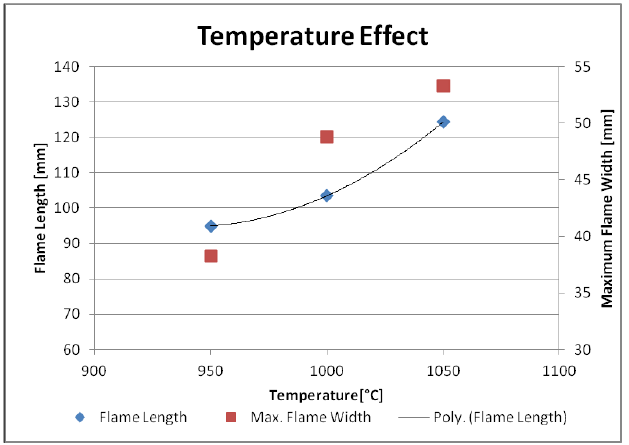
\includegraphics[width=0.45\textwidth]{fig/Optisos_temperature_effect.PNG}
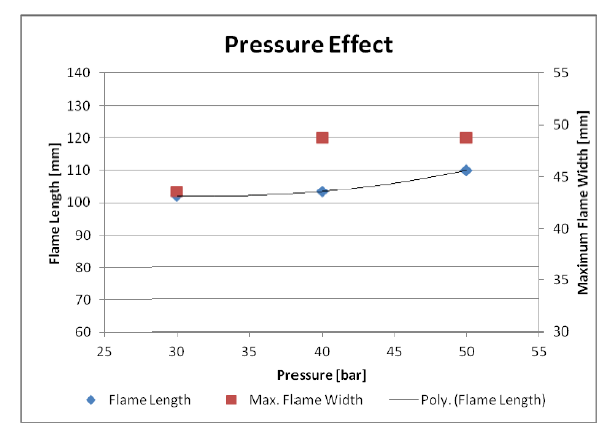
\includegraphics[width=0.45\textwidth]{fig/Optisos_Pressure_effect.PNG}
  \caption{Conclusion of Optisos report on flame topology}
 \label{optisos_plot}
\end{figure}

Dealing with my internship, if the flame length depended on so many parameters, it mean that I would have to study them all, and to keep them constant in Calhory burner with scales-up rule. This task seems impossible to achieve. Besides, a analysis of  the literature gives another interpretation. 

In a the laminar case : in (\# ref Veynante), the length of a diffusion flame in the laminar case is $L_{f}=\frac{e_{0}Re}{2\pi}\cdot \frac{1}{Z_{st}^2}$  with $e_{0}$ a geometrical length. With  $Z_{st}=(1+\frac{\nu Y_{F,1}}{Y_{O_{2},2}})^{-1}$ where $\nu$ is the mass stoechiometric ratio (4 for $CH_{4}-O_{2}$ flame),    $Y_{F,1}$ the mass ratio of fuel in the fuel injection ($Y_{F,1}=1$ if it is pure $CH_{4}$) and $Y_{O_{2},2}$ the mass ratio of oxygen in the oxidant injection ($Y_{O_{2},2}=0.23$ if it is pure air). 

In an analysis from (\# ref Peters), in a case with static oxidant and a non swirled fluel flow, Peters demonstrates the flame length :$\frac{L+x_{0}}{d}=\frac{2.19 (1+2Sc)}{Z_{st}}\frac{\rho_{0}}{\rho_{st}C}$, while another (\# ref) gets experimentally the length  $\frac{L+x_{0}}{d}=\frac{5.3}{Z_{st}}(\frac{\rho}{\rho_{st}})^{-1/2}$.

The purpose of these formulas is obviously not to use them for a much more complicated case (swirled coaxial flow), but to consider that all the parametric parameters studied in Optisos report can be gathered with adimensional number. If these formula were correct, the flame length should depend on the stoichiometric mixture fraction $Z_{st}$, since $Z_{st}$ keeps all the information of S/C dilution, burner load or pressure variation of density.

Hence, the data from Optisos has been re-used to compute in each test the corresponding $Z_{st}$, and it has be found that, in the area of the tests that have been conducted, the flame length of ATR burner measured in Optisos diagnostic directly depends on the stoichiometric mixture fraction $Z_st$ as an affine function :

The points in red are the cases where the temperature of the reactor has been changed, which does not implicate the $Z_{st}$, and adresses heat transfer and kinetic.

\begin{figure}[h!]
  \centering
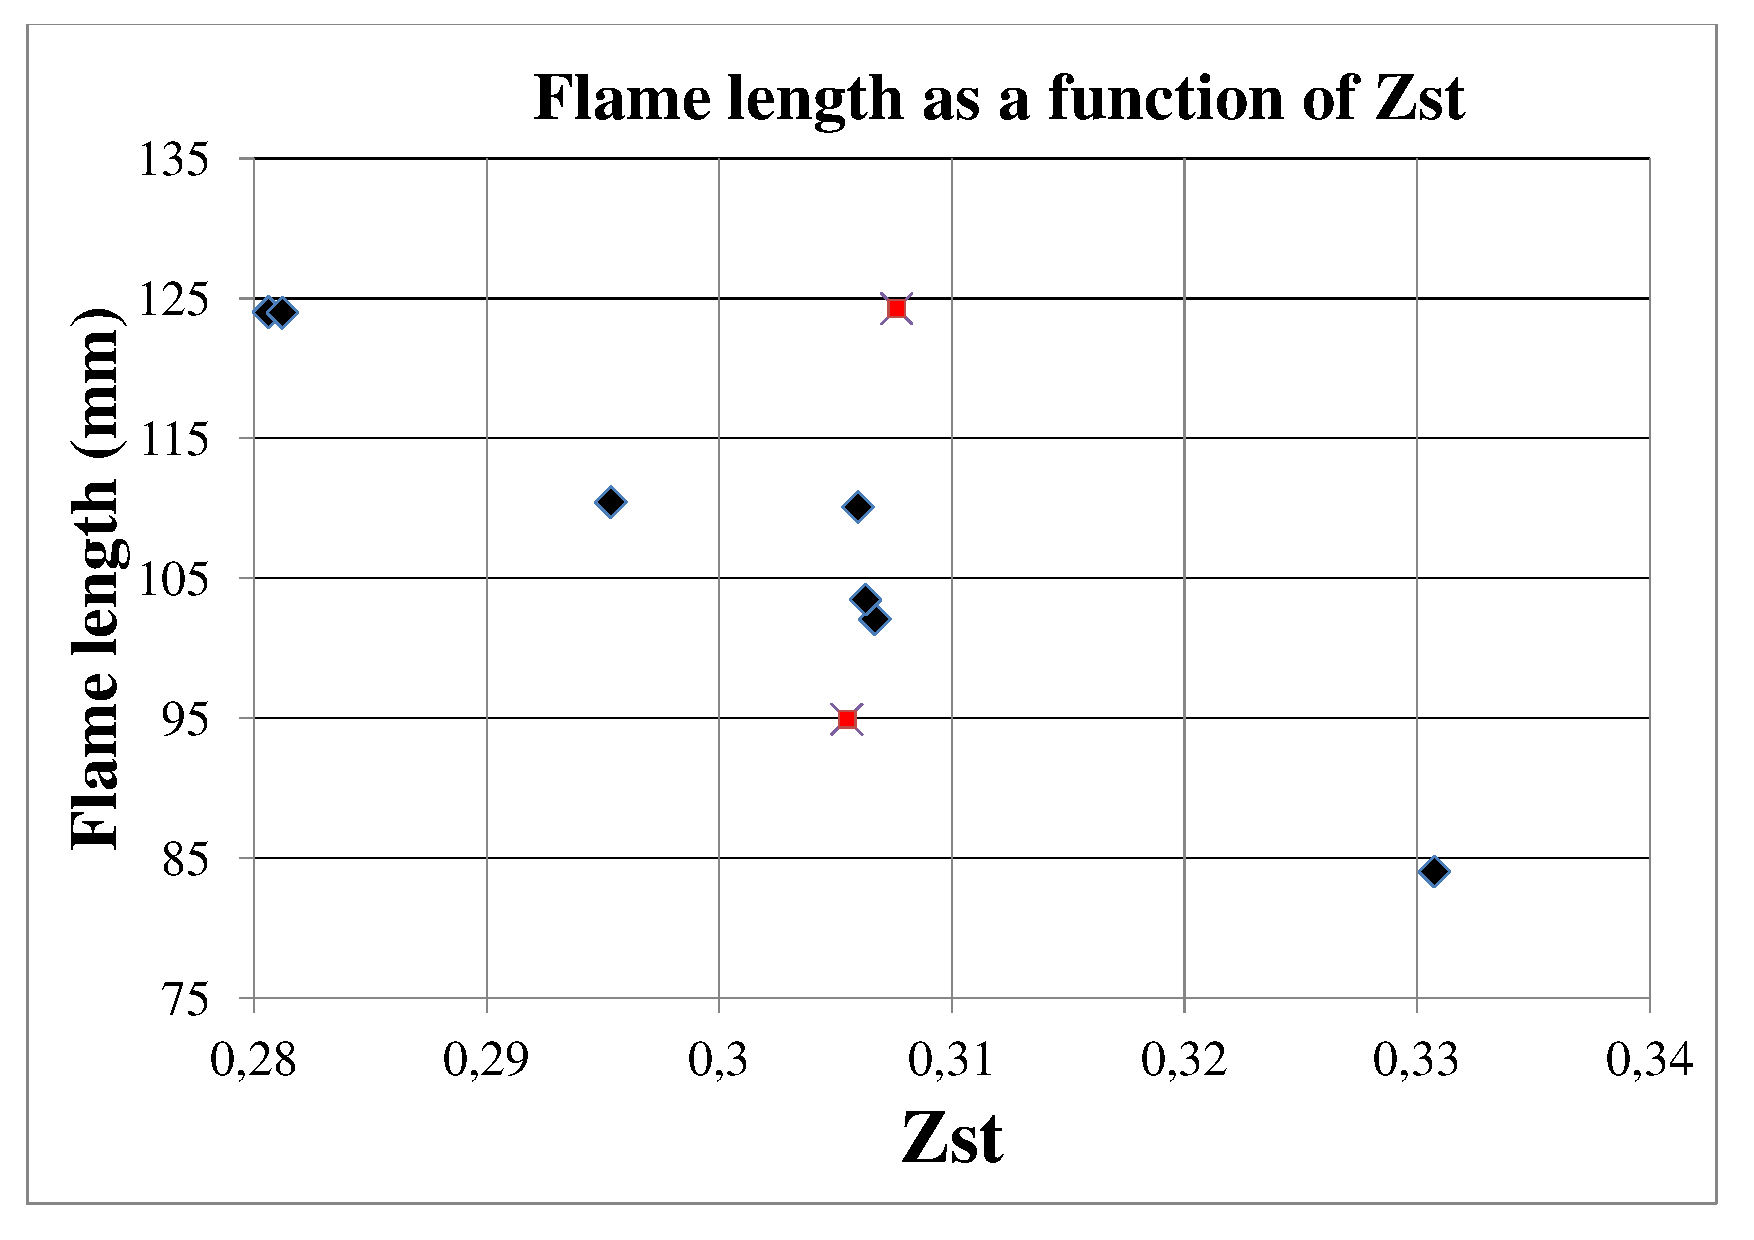
\includegraphics[width=0.8\textwidth]{fig/Flame_length_Zst.pdf}
 \label{Flame length as a function of Zst}
\end{figure}

It would be interested to get more points, or to extend the investigation segment, to define a characteristic law such as $Length=A_{0}-A_{1}\cdot Z_{st}$. One can easily verify that the trend is logical according to what have been observed previously, 